\begin{abstract}
Generative models increasingly sit inside data pipelines rather than at the end, aligning
data from different sources or manufacturing training examples. They are picked by asking
whether outputs resemble the data we want. The failure is built into that question. The
audit is simple: freeze the model that consumes the data, score it alongside the resemblance
score on identical inputs, and add a control with no learned prior. Passing data through a
learned transform erases information the task needs while resemblance improves. The damage
belongs to the objective, not an architecture: it holds for both adversarial and diffusion
generators, grows with how much of the transform is applied, survives constraints meant to
preserve structure, and persists even when resemblance worsens. The mechanism is
selectivity: distribution matching rewards reproducing common patterns while rare ones are
overwritten, and rare ones often carry the label. Without a learned prior nothing is
substituted, and the task survives. Two unrelated fields, driving and clinical, behave
identically: harmonizing hospital scans toward the sites a tumor segmenter was trained on
drops its accuracy from 0.68 to 0.06, while plain normalization holds 0.67. The data looks
better; the model has stopped working. One frozen model and one control catch this before
deployment.
\end{abstract}

\section{Introduction}
Generative models increasingly sit \emph{inside} data pipelines rather than at their end:
they align data collected under different conditions, or manufacture training examples
outright. Practitioners choose among them by asking how closely the output resembles the
data they want, typically with a distributional metric such as the Fr\'echet Inception
Distance (FID). The implicit promise is that a closer match makes the data more
\emph{useful} to whatever consumes it downstream. We test that promise directly and find it
false whenever the transform is learned: the resemblance score improves while the
information the downstream task depends on is destroyed. Because the metric being optimised
is precisely the one that cannot see the damage, the failure is silent.

Our contributions are:
\begin{itemize}
  \item A \textbf{controlled protocol} for separating fidelity from utility: a
  frozen downstream evaluator plus a matched non-learned control, measuring FID
  and the task metric on identical inputs (Section~\ref{sec:setup}).
  \item Evidence that the fidelity--utility dissociation is a property of the
  \textbf{learned distribution-matching objective}, not a single architecture---it
  reproduces under both a GAN (CycleGAN) and a diffusion model (SDEdit).
  \item A \textbf{continuous characterization} via SDEdit strength: a monotonic
  FID-vs-mIoU frontier with tight seed variance, an empty-prompt ablation that
  decouples utility loss from fidelity gain, and a structure-preserving
  (ControlNet) baseline that fails to escape the frontier.
  \item \textbf{Cross-domain} generality: the same dissociation in driving scenes
  and in clinical brain-tumor MRI.
\end{itemize}

\section{Related Work}
Three separately-established observations converge in our claim; we unify them.

\paragraph{Fidelity metrics mis-rank generators for downstream tasks.}
\citet{konz2024rethinking} show no perceptual metric reliably tracks segmentation
quality in medical translation; \citet{dutt2025chexgenbench} show low FID does not
predict clinical utility; and \citet{kynkaanniemi2023role} show FID is gameable by
aligning ImageNet-class statistics. These are \emph{metric-evaluation} studies; we
add a learned/non-learned control and a second generative family and domain.

\paragraph{Distribution-matching translation alters task content.}
\citet{cohen2018distribution} show CycleGAN-style matching can hallucinate or
remove tumors to fit the target distribution, and semantic-consistency losses
\citep{hoffman2018cycada,peng2023diffusion} exist precisely to patch this. We show
that \emph{without} such non-distributional anchoring the pure learned objective
degrades utility, reframing those losses as evidence for our thesis.

\paragraph{Non-learned alignment rivals learned translation.}
\citet{yang2020fda} reach strong segmentation adaptation with a non-learned
spectral swap. We use histogram/color transfer as the analogous control and,
unlike FDA, measure the fidelity axis explicitly to expose the dissociation.
\citet{richter2022enhancing} likewise treat a segmentation-stability metric as a
guardrail that realism must not break.

\paragraph{Positioning.} No prior work runs the clean $2\times2$
$\{$learned, non-learned$\}\times\{$fidelity$\downarrow?$, utility$\downarrow?\}$
as its thesis, ties the failure to the objective across both a GAN \emph{and} a
diffusion model, and does so across driving and medicine. This is a
measurement/positioning contribution, not a new architecture.

\section{Setup: Separating Fidelity from Utility}
\label{sec:setup}
Given source images $x$ and a translation $T$, we evaluate $T(x)$ on two axes.
\textbf{Fidelity} is $\mathrm{FID}(T(x),\text{target})$ via
clean-fid~\citep{parmar2022cleanfid}; lower is closer to the target.
\textbf{Utility} is a \emph{frozen} downstream model $f$ (never retrained) applied
to $T(x)$ and scored against ground truth; because $f$ is fixed, any change in its
score is attributable purely to $T$. We compare four families of $T$:
(i) identity (raw source, reference); (ii) non-learned (histogram / color
transfer); (iii) learned-GAN (CycleGAN, \citealp{zhu2017cyclegan}); and
(iv) learned-diffusion (SDEdit, \citealp{meng2022sdedit}, over a sweep of noise
strengths, plus ControlNet-Canny, \citealp{zhang2023controlnet}). FID is compared
only at equal sample size, which it is known to bias.

\section{Experiments}

\subsection{Driving: GTA5 $\rightarrow$ Cityscapes}
The source is GTA5~\citep{richter2016playing} and the target is
Cityscapes~\citep{cordts2016cityscapes}. The frozen evaluator is a
Cityscapes-finetuned SegFormer-b4~\citep{xie2021segformer} (19 classes); utility is
mIoU. We use $N{=}1000$ GTA5 images per condition, with the Cityscapes validation
set (500 images) as the fixed FID reference, and identical evaluator and clean-fid
(GPU) for all conditions. SDEdit runs on Stable Diffusion~\citep{rombach2022ldm}
and rows report mean $\pm$ std over three seeds $\{42,43,44\}$. Results are in
Table~\ref{tab:driving} and Figure~\ref{fig:frontier}.

\begin{table}[t]
\centering
\caption{GTA5$\rightarrow$Cityscapes, $N{=}1000$, frozen SegFormer-b4 + clean-fid.
SDEdit rows are mean $\pm$ std over three seeds. Learned translation lowers FID
while collapsing mIoU; the non-learned baseline preserves mIoU without improving
FID; no learned setting reaches the low-FID/high-mIoU corner.}
\label{tab:driving}
\begin{tabular}{llrrr}
\toprule
condition & family & FID $\downarrow$ & mIoU $\uparrow$ & $\Delta$mIoU \\
\midrule
raw GTA5 & baseline & 137.2 & 0.380 & --- \\
color match & non-learned & 165.9 & 0.363 & $-0.018$ \\
SDEdit 0.20 & diffusion & $145.1{\pm}1.8$ & $0.323{\pm}0.003$ & $-0.057$ \\
SDEdit 0.30 & diffusion & $133.1{\pm}2.1$ & $0.289{\pm}0.002$ & $-0.092$ \\
SDEdit 0.40 & diffusion & $116.4{\pm}1.1$ & $0.237{\pm}0.003$ & $-0.143$ \\
SDEdit 0.50 & diffusion & $100.3{\pm}1.4$ & $0.194{\pm}0.005$ & $-0.187$ \\
SDEdit 0.60 & diffusion & $90.8{\pm}2.0$ & $0.150{\pm}0.001$ & $-0.231$ \\
SDEdit 0.70 & diffusion & $88.0{\pm}0.4$ & $0.106{\pm}0.001$ & $-0.274$ \\
CycleGAN & learned-GAN & 65.5 & 0.167 & $-0.214$ \\
SDEdit 0.50, empty prompt & diffusion (abl.) & $154.2{\pm}1.9$ & $0.170{\pm}0.003$ & $-0.211$ \\
ControlNet-Canny & diffusion + edge & $133.2{\pm}0.3$ & $0.221{\pm}0.002$ & $-0.159$ \\
\bottomrule
\end{tabular}
\end{table}

\begin{figure}[t]
\centering
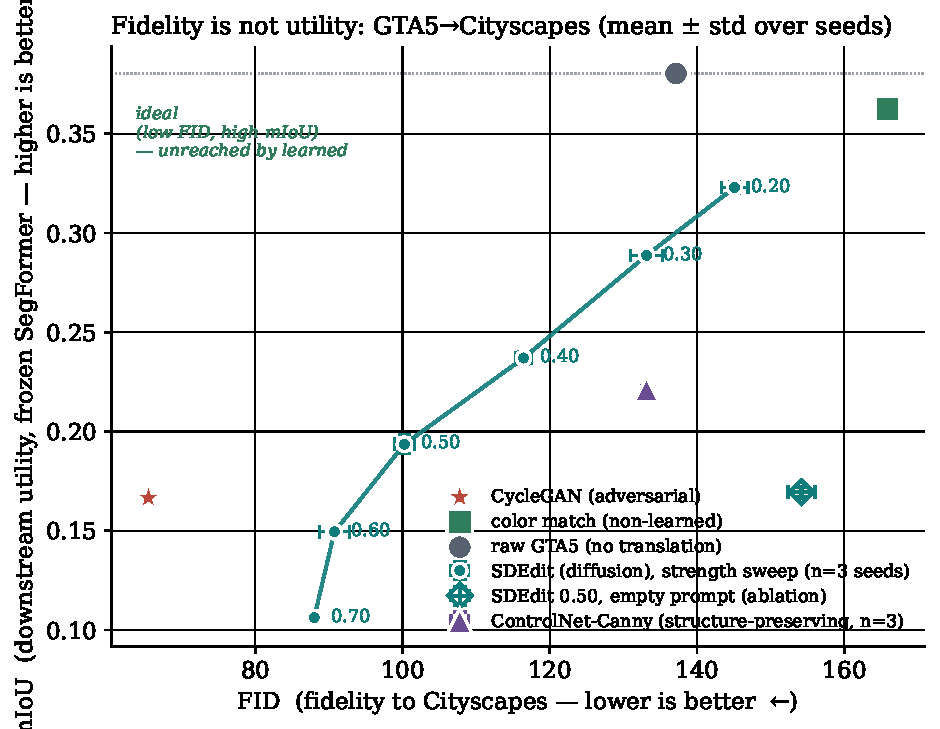
\includegraphics[width=0.72\linewidth]{frontier_seeds.pdf}
\caption{The fidelity--utility plane for GTA5$\rightarrow$Cityscapes (mean $\pm$
std over seeds). The SDEdit strength sweep traces a monotonic frontier: as strength
rises, FID falls and mIoU falls with it. Every learned point (CycleGAN, all SDEdit
strengths, the empty-prompt ablation, and edge-conditioned ControlNet) sits well
below raw and the non-learned baseline on utility; the ideal low-FID/high-mIoU
corner is empty.}
\label{fig:frontier}
\end{figure}

\begin{figure}[t]
\centering
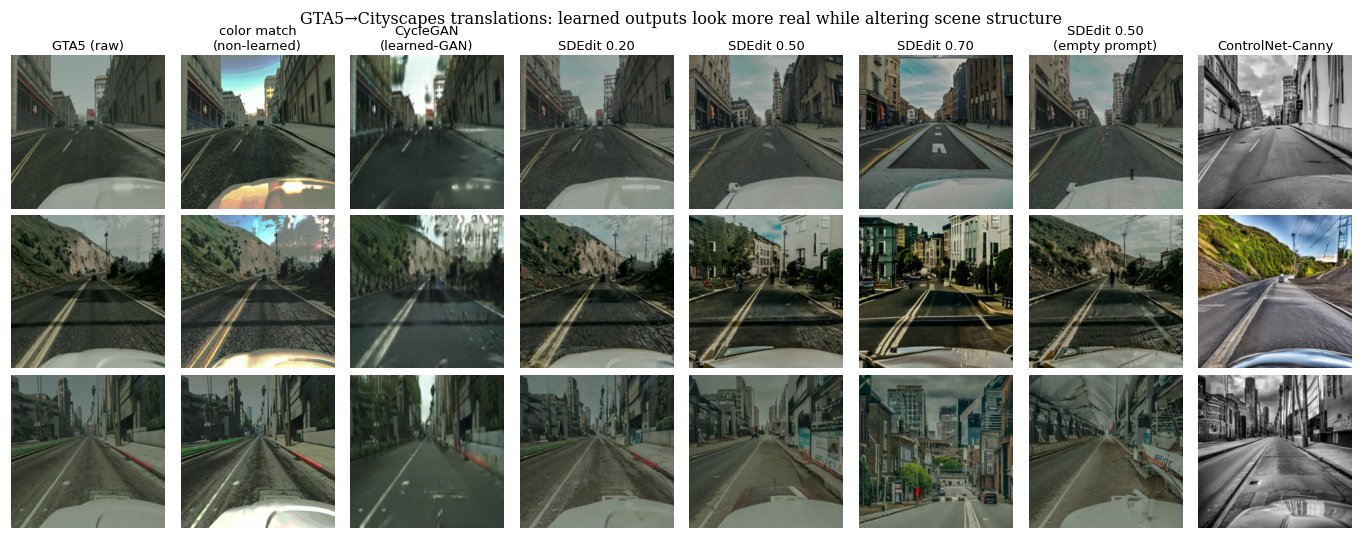
\includegraphics[width=\linewidth]{qualitative.jpg}
\caption{Qualitative GTA5$\rightarrow$Cityscapes translations (three scenes, seed 42). Left to right: raw
source, non-learned color match, CycleGAN, SDEdit at increasing strength, the empty-prompt SDEdit, and
edge-conditioned ControlNet. As the learned translations become more Cityscapes-like they visibly
hallucinate and alter scene structure---buildings, lane markings, added objects---that the frozen
segmenter depends on, while the non-learned baseline leaves structure intact.}
\label{fig:qualitative}
\end{figure}

\paragraph{Findings.}
Figure~\ref{fig:qualitative} shows representative translations.
(a) Learned translation lowers FID relative to raw while collapsing mIoU by
15--72\%; CycleGAN more than halves FID ($137{\rightarrow}65$) at mIoU 0.167.
(b) The non-learned baseline does not improve FID yet preserves mIoU ($-1.8\%$).
(c) SDEdit strength traces a \textbf{monotonic frontier} with tight seed variance
($\sigma(\text{mIoU})\le 0.005$): as strength rises, FID falls ($145{\rightarrow}88$)
and mIoU falls with it ($0.323{\rightarrow}0.106$); no learned setting reaches the
ideal corner, occupied only by raw/non-learned.
(d) \textbf{Empty-prompt ablation.} With no text prompt, FID is \emph{worse} than
raw ($154.2 > 137.2$) yet mIoU still collapses ($0.170$)---the utility loss is the
diffusion prior itself, not text guidance, and occurs even absent any fidelity gain.
(e) \textbf{Structure-preserving baseline.} Conditioning on the source image's
Canny edges (ControlNet-Canny) does \emph{not} rescue utility: it lands on the
learned frontier (FID 133.2, mIoU $0.221{\pm}0.002$), Pareto-dominated by SDEdit at
equal FID (SDEdit 0.30: FID 133.1, mIoU 0.289). Edge structure is not the
task-relevant signal; only conditioning on the segmentation \emph{map}
\citep{peng2023diffusion} recovers utility, and only by injecting the labels---the
non-distributional constraint our thesis requires. A local $N{=}200$ run reproduces
the same ordering on an independent machine.

\subsection{Medical: Multi-Site Brain-Tumor MRI}
The frozen evaluator is an nnU-Net~\citep{isensee2021nnunet} trained on
BraTS~\citep{menze2015brats} and frozen; utility is tumor Dice on the external
UPenn-GBM site~\citep{bakas2022upenn} ($n{=}103$). The learned harmonizer is
SA-CycleGAN-2.5D, a self-attention CycleGAN over 2.5D multi-modal MRI.
Table~\ref{tab:medical} reports the result.

\begin{table}[t]
\centering
\caption{External UPenn-GBM tumor Dice under a frozen BraTS-trained nnU-Net.
Learned harmonization collapses Dice even though it makes images more source-like;
the non-learned baseline preserves it.}
\label{tab:medical}
\begin{tabular}{llr}
\toprule
input to frozen nnU-Net & family & Dice (fg. mean) \\
\midrule
BraTS test (in-domain ref.) & --- & 0.771 \\
UPenn raw (external) & baseline & 0.682 \\
UPenn + histogram match & non-learned & 0.669 \\
UPenn + learned harmonization & learned-GAN & 0.064 \\
UPenn + symmetric seg-consistency & learned-GAN (+ content) & 0.205 \\
\bottomrule
\end{tabular}
\end{table}

\paragraph{Findings.} Learned harmonization collapses external-site Dice
($0.682{\rightarrow}0.064$) while the non-learned baseline preserves it ($0.669$).
Content/segmentation-consistency losses reduce but do not eliminate the loss
($0.205 \ll 0.682$), consistent with the driving result that the degradation is
intrinsic to the learned objective. A second external site (RHUH-GBM,
\citealp{cardoso2022rhuh}, $n{=}40$) confirms the direction
($0.718{\rightarrow}0.599$, $-16.6\%$). We note two evaluation protocols exist: the
headline numbers use the frozen independent nnU-Net; a separate
method-development evaluator ranks the symmetric loss as the best-preserving
\emph{learned} harmonizer, which belongs to a companion method paper.


\subsection{Where the damage falls}
\label{sec:perclass}
The headline mIoU collapse hides structure. Breaking IoU out per class and grouping the 19
Cityscapes classes into large amorphous regions and thin, small, label-carrying objects
(Table~\ref{tab:perclass}) shows the degradation is highly \emph{selective}. The non-learned
control loses a few percent on both groups, almost uniformly. Every learned translation instead
loses far more on the thin classes than on the large ones: SDEdit at strength 0.50 costs 27\% of
large-region IoU but 83\% of thin-object IoU, and CycleGAN 50\% against 70\%. Poles, traffic
lights, traffic signs, riders and motorcycles are precisely the structures a segmenter needs and
precisely what the learned prior does not preserve. Edge-conditioned ControlNet sits in between
(27\% / 63\%): conditioning on edges recovers some thin structure, consistent with
Section~\ref{sec:setup}'s argument that what is missing is a non-distributional constraint, but
not enough to escape the frontier.

\begin{table}[t]
\centering
\caption{Per-class IoU grouped into large amorphous regions (road, sidewalk, building,
vegetation, terrain, sky) and thin/small label-carrying objects (pole, traffic light, traffic
sign, rider, motorcycle); classes whose raw IoU is below $0.05$ are excluded, since a ratio off a
near-zero baseline is noise. The non-learned control degrades both groups mildly and almost
uniformly; every learned translation degrades the thin classes far more than the large ones.}
\label{tab:perclass}
\begin{tabular}{lrrrrr}
\toprule
group & raw & color match & CycleGAN & SDEdit 0.50 & ControlNet \\
\midrule
large regions        & 0.661 & 0.630 ($-5\%$)  & 0.328 ($-50\%$) & 0.481 ($-27\%$) & 0.482 ($-27\%$) \\
thin / small objects & 0.174 & 0.168 ($-4\%$)  & 0.052 ($-70\%$) & 0.030 ($-83\%$) & 0.065 ($-63\%$) \\
\bottomrule
\end{tabular}
\end{table}

\section{Analysis}
The learned objective optimizes appearance under a distribution/adversarial or
denoising target with no term guaranteeing task-relevant signal survives. SDEdit
strength is precisely the amount of learned prior injected, and utility falls
monotonically with it. The empty-prompt result decouples utility loss from fidelity
gain: passing through the prior damages task content even when the output is
\emph{less} target-like. Non-learned transforms, lacking a learned prior, cannot
introduce this failure; edge-conditioned ControlNet, injecting structure but not
semantics, does not avoid it.

\section{Limitations}
FID is sample-size biased; all conditions use the same $N$ (1000 translated vs the
500-image Cityscapes validation set as the fixed reference), and SDEdit points
report mean $\pm$ std over three seeds ($\sigma(\text{mIoU})\le0.005$,
$\sigma(\text{FID})\le2.1$), so the ordering is robust to both sample size and
seed. The structure-preserving baseline uses edge (Canny) conditioning; a
segmentation-map-conditioned variant would recover utility only by injecting the
labels, which concedes the thesis rather than refuting it.

\section{Conclusion}
Fidelity is not utility. Rewarding distributional realism can actively harm the
downstream task for learned translation, across architectures and domains. We
recommend reporting a frozen-evaluator utility axis alongside any fidelity metric,
and treating non-learned baselines as first-class controls.

\section*{Reproducibility Statement}
All conditions regenerate from a single command; seeds are fixed and logged; frozen
evaluators are referenced by checkpoint id (SegFormer-b4, nnU-Net); FID uses
clean-fid at a fixed $N$. Code, configs, and the $N{=}1000$ result set are released
with the paper.

\appendix
\section{Full per-class IoU}
\label{app:perclass}
Table~\ref{tab:perclass-full} reports every Cityscapes class, the breakdown behind
Table~\ref{tab:perclass}. SDEdit and ControlNet columns are means over the three seeds. Classes
with very small raw IoU (\emph{train}, \emph{bicycle}) are near-absent in the GTA5 subset; a
relative change computed off such a baseline is noise, which is why the grouped statistics in
Table~\ref{tab:perclass} exclude classes with raw IoU below $0.05$. The selectivity is visible
directly: \emph{road} loses little under every condition, while \emph{traffic light},
\emph{traffic sign}, \emph{person} and \emph{rider} are almost entirely destroyed by the learned
translations and almost untouched by the non-learned control.

\begin{table}[h]
\centering
\caption{Per-class IoU under a frozen SegFormer-b4, $N{=}1000$.}
\label{tab:perclass-full}
\begin{tabular}{lrrrrr}
\toprule
class & raw & color match & CycleGAN & SDEdit 0.50 & ControlNet \\
\midrule
road & 0.937 & 0.932 & 0.843 & 0.845 & 0.884 \\
sidewalk & 0.540 & 0.502 & 0.202 & 0.280 & 0.309 \\
building & 0.711 & 0.681 & 0.356 & 0.504 & 0.505 \\
wall & 0.356 & 0.315 & 0.089 & 0.077 & 0.094 \\
fence & 0.102 & 0.111 & 0.020 & 0.021 & 0.031 \\
pole & 0.269 & 0.252 & 0.112 & 0.095 & 0.159 \\
traffic light & 0.073 & 0.067 & 0.008 & 0.008 & 0.012 \\
traffic sign & 0.069 & 0.063 & 0.012 & 0.017 & 0.022 \\
vegetation & 0.649 & 0.625 & 0.364 & 0.455 & 0.427 \\
terrain & 0.227 & 0.159 & 0.083 & 0.050 & 0.011 \\
sky & 0.901 & 0.883 & 0.121 & 0.750 & 0.755 \\
person & 0.270 & 0.240 & 0.035 & 0.024 & 0.111 \\
rider & 0.182 & 0.156 & 0.028 & 0.015 & 0.085 \\
car & 0.737 & 0.725 & 0.384 & 0.226 & 0.447 \\
truck & 0.666 & 0.608 & 0.198 & 0.197 & 0.175 \\
bus & 0.248 & 0.259 & 0.206 & 0.097 & 0.127 \\
train & 0.002 & 0.002 & 0.000 & 0.001 & 0.001 \\
motorcycle & 0.279 & 0.303 & 0.101 & 0.016 & 0.046 \\
bicycle & 0.008 & 0.007 & 0.001 & 0.001 & 0.004 \\
\bottomrule
\end{tabular}
\end{table}
